\section{Calorimeter}\label{sec:calorimeter}

The LXe calorimeter is a homogenous calorimeter using liquid Xenon scintillator
enclosed in a semi-cylindrical (C-shaped) volume placed around the COBRA magent
\cite{megdesign}.  It is designed to detect prompt scintialltion light from
photons originating in \muon decays, interacting at LXe temperature 170~K in the
VUV range ($\lambda = 175 \pm 5$ nm).  The surface of the enclosed volume is
covered with two different photodetectors, the inner face  with MPPC and the
rest of the surfaces with 2-inch PMT.  The axis of the cylindrical calorimeter
is nominally aligned with the Z axis in MEG coordinate system.

The inner face of the LXe calorimeter consists of 4092 MPPCs arranged in a grid
structure containing 93 rows in the $\phi$ direction.  A row consists of 44
MPPCs placed along $\hat{z}$ direction, divided equally in two PCB\footnote{Printed
Circuit Board} strips, placed on the upstream ($Z<0$ mm) and downstream ($Z>0$
mm) sides of the calorimeter.  The PCB strips are mounted with spacer materials
on four CFRP\footnote{Carbon Fiber Reinforced Polymer} plates, each containing
23-24 strips and attached to the inner face of the cryostat at different $\phi$
locations.  
\begin{figure}
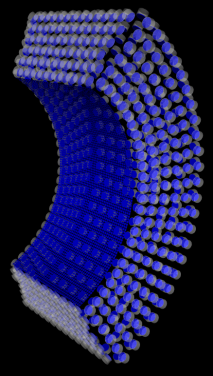
\includegraphics[height=4cm]{plots/LXeMEGUpgrade.png}
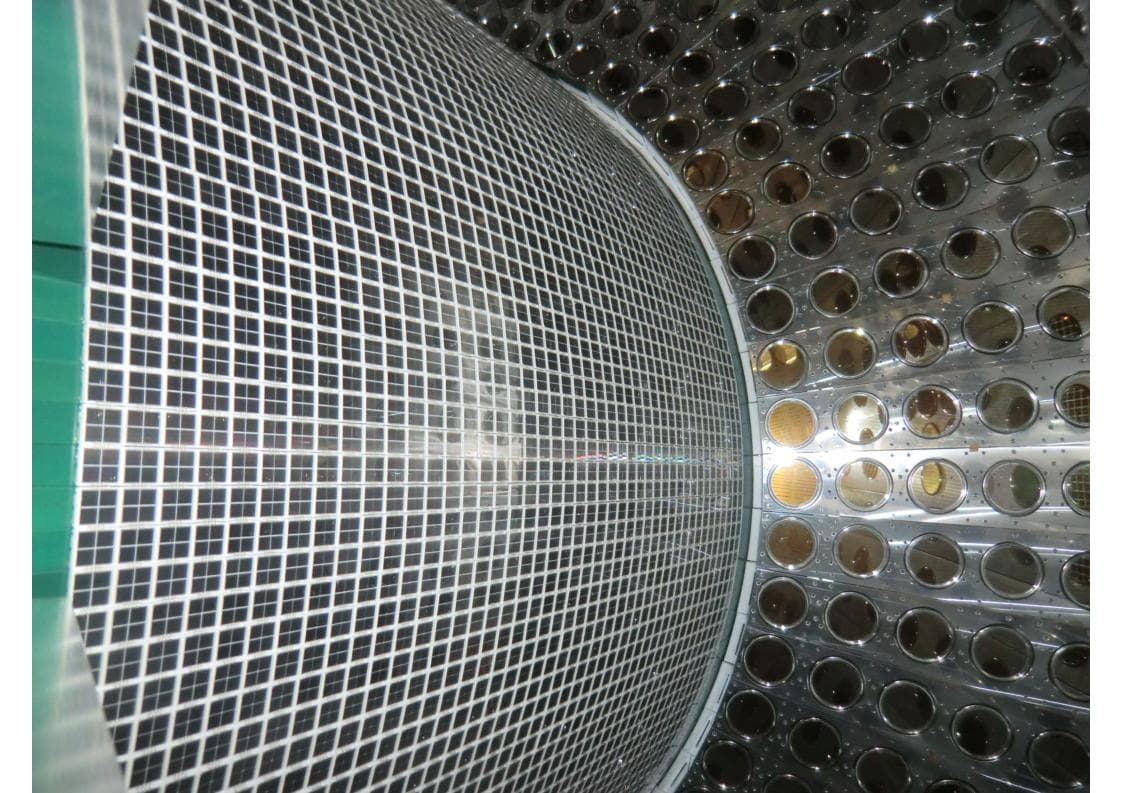
\includegraphics[height=4cm]{plots/CIMG5301}
\label{fig:calorimeter}
\caption{Liquid Xe calorimeter in the MEG experiment.}
\end{figure}
The MPPC photodetectors are developed according to the experimental
requirements with large photosensitive area 12 $\times$ 12 mm$^2$,
comprised of four  smaller pixels 6 $\times$ 6 mm$^2$ connected in
series.  The photodetectors are placed in a ceramic case (15 mm) and
mounted on a PCB strip, each containing 22 photodetectors.  Two
identically produced strips aligned along $\hat{z}$ direction, and
rotated by 180\degree with respect to each other to allow for
electronics readout at each end, make up a single row (fig 
\ref{fig:mppc}).
\begin{figure}
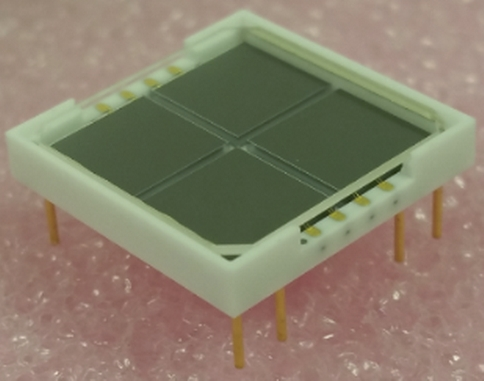
\includegraphics[width=3cm]{plots/single_mppc.jpg}
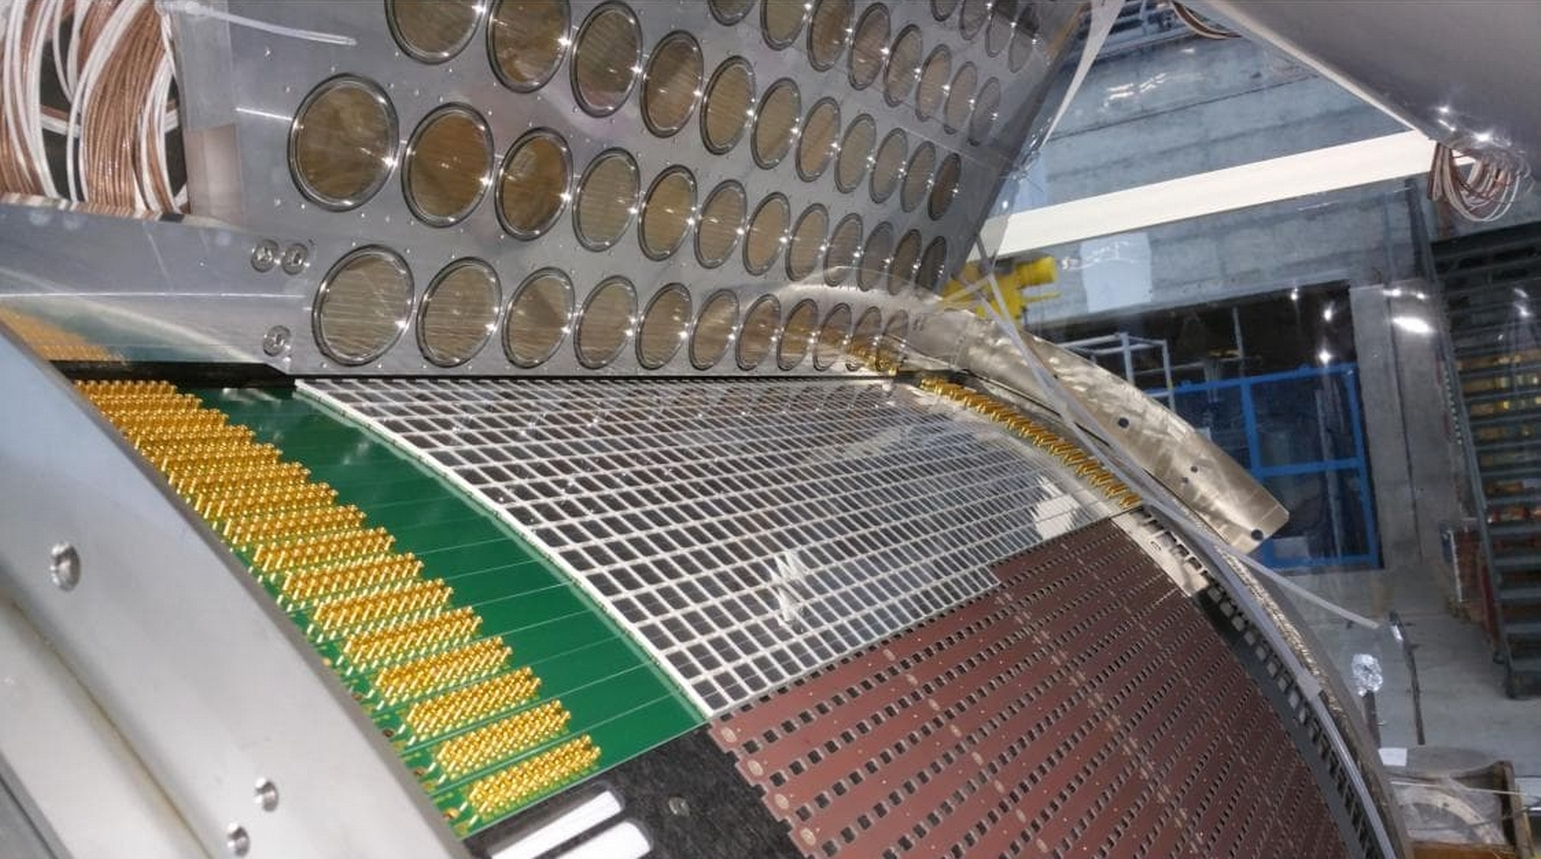
\includegraphics[width=5cm]{plots/CFRP_spacer_MPPC.jpg}
\caption{Single MPPC and installed MPPCs in the LXe calorimeter.}
\label{fig:mppc} 
\end{figure}


